\documentclass[10pt,a4paper,twocolumn]{article}

% ---------------------------------------------------------------- pacchetti
\usepackage[T1]{fontenc}
\usepackage[utf8]{inputenc}
\usepackage{babel}
\babelprovide[import,main]{italian}
\usepackage{mathptmx}                 % Times, aspetto da paper
\usepackage[scaled=0.86]{helvet}
\usepackage{microtype}
\usepackage[a4paper,top=2cm,bottom=2.2cm,left=1.8cm,right=1.8cm,columnsep=0.75cm]{geometry}
\usepackage{amsmath}
\usepackage{booktabs,tabularx,multirow}
\usepackage[table]{xcolor}
\usepackage{caption}
\usepackage{enumitem}
\usepackage{titlesec}
\usepackage{listings}
\usepackage{pgfplots}
\pgfplotsset{compat=1.16}
\usetikzlibrary{positioning,arrows.meta,shapes.geometric}
\usepackage{fancyhdr}
\usepackage[hidelinks]{hyperref}
\usepackage[italian,nameinlink]{cleveref}

% ---------------------------------------------------------------- stile
\definecolor{accento}{RGB}{31,56,100}
\definecolor{stdcol}{RGB}{150,150,150}
\definecolor{itacol}{RGB}{31,90,160}
\definecolor{grigiochiaro}{RGB}{245,245,245}

\titleformat{\section}{\normalfont\sffamily\bfseries\large\color{accento}}{\thesection.}{0.5em}{}
\titleformat{\subsection}{\normalfont\sffamily\bfseries\color{accento}}{\thesubsection}{0.5em}{}
\titlespacing*{\section}{0pt}{1.2ex plus .5ex}{0.6ex}
\titlespacing*{\subsection}{0pt}{1ex plus .3ex}{0.4ex}

\captionsetup{font=small,labelfont={bf,sf},labelsep=period}
\setlist{nosep,leftmargin=*,topsep=2pt}
\lstset{basicstyle=\ttfamily\footnotesize,backgroundcolor=\color{grigiochiaro},
        frame=none,breaklines=true,columns=fullflexible,xleftmargin=2pt}

\pagestyle{fancy}
\fancyhf{}
\renewcommand{\headrulewidth}{0.4pt}
\fancyhead[L]{\small\sffamily Ingegneria dei Dati -- Homework 3}
\fancyhead[R]{\small\sffamily C. Nota}
\fancyfoot[C]{\small\thepage}

\setlength{\emergencystretch}{1.5em}
\newcommand{\file}[1]{\texttt{#1}}
\newcommand{\cls}[1]{\textsf{#1}}

% ---------------------------------------------------------------- titolo
\title{\sffamily\bfseries\color{accento}Indicizzazione e ricerca full-text di file di testo con Apache Lucene:\\[2pt]
\Large un confronto tra analyzer su un corpus di libri italiani}
\author{%
  \textbf{Carlo Nota}\\
  \small Università degli Studi Roma Tre -- matricola 561636\\
  \small\href{mailto:car.nota@stud.uniroma3.it}{car.nota@stud.uniroma3.it}\\
  \small Codice: \url{https://github.com/carlo0o0o/IDD.HW3}}
\date{\small Novembre 2026}

\begin{document}

\twocolumn[
\begin{@twocolumnfalse}
\maketitle
\thispagestyle{fancy}
\begin{center}
\begin{minipage}{0.86\textwidth}
\small
\noindent\textbf{\sffamily Sommario.}
Presentiamo un sistema di indicizzazione e ricerca di file \file{.txt} basato su Apache Lucene, con due campi
(nome del file e contenuto) e un analyzer dedicato a ciascuno. Il corpus, costruito da 15 libri italiani di
Project Gutenberg, conta 2365 documenti e circa 1,9 milioni di parole; viene indicizzato in circa 3 secondi.
Confrontiamo due configurazioni per il campo contenuto, \cls{StandardAnalyzer} e \cls{ItalianAnalyzer}, su 14
query di test con un ground truth esplicito e indipendente da Lucene. \cls{ItalianAnalyzer} riduce l'indice del
26--29\% e porta la recall media da 0,804 a 0,870 (da 0,61 a 0,74 sulle query sensibili alle varianti delle
parole), con un lieve calo di precision sulle frasi esatte. L'analisi dei casi scoperti (accenti, coniugazioni,
elisioni) indica le estensioni da sperimentare.

\smallskip
\noindent\textbf{\sffamily Parole chiave:} information retrieval, Apache Lucene, analyzer, stemming, valutazione, precision, recall.
\end{minipage}
\end{center}
\vspace{1.2em}
\end{@twocolumnfalse}
]

% =================================================================
\section{Introduzione}
Il compito richiede di indicizzare i file di testo contenuti in una cartella considerando due campi, il nome e il
contenuto del file, con un analyzer appropriato per ciascuno; di interrogare l'indice da console con una
sintassi semplice, che includa le phrase query; e di valutare il sistema con un insieme di query di test.

Oltre a soddisfare questi requisiti, il lavoro si propone di \emph{motivare con i dati} la scelta degli
analyzer. Per questo abbiamo costruito un corpus abbastanza grande da rendere significativi i tempi di
indicizzazione e la recall, definito un ground truth in modo esplicito e confrontato due configurazioni sulle
stesse query con metriche standard~\cite{manning2008}.

% =================================================================
\section{Architettura del sistema}
Il sistema (\cref{fig:arch}) è composto da un progetto Maven in Java, basato su Apache Lucene 9.12.1~\cite{lucene},
e da due script Python per la preparazione dei dati:
\begin{itemize}
  \item \file{prepara\_corpus.py} scarica, pulisce e divide i libri in documenti;
  \item \cls{Indicizzatore} costruisce l'indice e ne misura i tempi;
  \item \cls{Ricerca} è il programma interattivo da console;
  \item \file{ground\_truth.py} calcola i documenti rilevanti di ogni query;
  \item \cls{Valutazione} esegue le query e calcola le metriche.
\end{itemize}
Gli esperimenti sono stati eseguiti su un laptop Windows, con la JRE integrata in Eclipse (OpenJDK 21) e Python~3.

\begin{figure}[t]
\centering
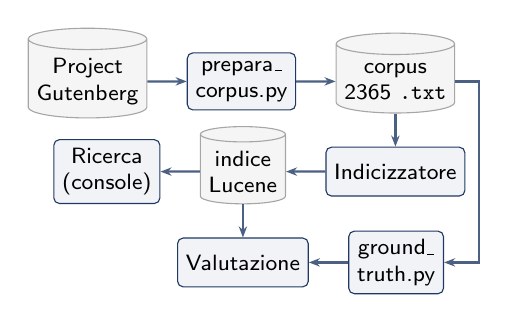
\begin{tikzpicture}[
  node distance=0.42cm and 0.5cm,
  box/.style={draw=accento,fill=accento!6,rounded corners=2pt,font=\footnotesize\sffamily,
              minimum height=0.62cm,align=center,inner sep=3pt},
  dato/.style={draw=gray!70,fill=gray!8,font=\footnotesize\sffamily,minimum height=0.55cm,
               align=center,inner sep=3pt,shape=cylinder,shape border rotate=90,aspect=0.18},
  freccia/.style={-{Stealth[length=4pt]},thick,accento!80}]
  \node[dato] (gut) {Project\\Gutenberg};
  \node[box, right=of gut] (prep) {prepara\_\\corpus.py};
  \node[dato, right=of prep] (corp) {corpus\\2365 \file{.txt}};
  \node[box, below=of corp] (idx) {Indicizzatore};
  \node[dato, left=of idx] (ind) {indice\\Lucene};
  \node[box, left=of ind] (ric) {Ricerca\\(console)};
  \node[box, below=of ind] (val) {Valutazione};
  \node[box, right=of val] (gt) {ground\_\\truth.py};
  \draw[freccia] (gut) -- (prep);
  \draw[freccia] (prep) -- (corp);
  \draw[freccia] (corp) -- (idx);
  \draw[freccia] (idx) -- (ind);
  \draw[freccia] (ind) -- (ric);
  \draw[freccia] (ind) -- (val);
  \draw[freccia] (corp.east) -- ++(0.3,0) |- (gt.east);
  \draw[freccia] (gt) -- (val);
\end{tikzpicture}
\caption{Architettura: dalla preparazione del corpus alla ricerca e alla valutazione.}
\label{fig:arch}
\end{figure}

% =================================================================
\section{Il dataset}
\label{sec:dataset}
Il corpus è formato da 15 libri in italiano di Project Gutenberg~\cite{gutenberg}, in pubblico dominio negli
Stati Uniti, scelti per coprire generi e registri molto diversi (\cref{tab:libri}): narrativa, poesia,
saggistica, storia, scienza, cucina, epistolario. La varietà di vocabolario rende le query discriminanti e
permette di definire in modo sensato la rilevanza.

Ogni libro è stato elaborato con i seguenti passi:
\begin{enumerate}
  \item rimozione di intestazione e licenza di Gutenberg (marker \texttt{START}/\texttt{END});
  \item divisione in capitoli o canti, se i titoli sono riconosciuti da un'espressione regolare, altrimenti in
        blocchi di circa 700 parole tagliati a fine paragrafo; pezzi sotto le 150 parole uniti al successivo,
        capitoli sopra le 3000 parole suddivisi in blocchi;
  \item salvataggio di ogni pezzo come file UTF-8 con nome nel formato \emph{libro-numero}, per esempio
        \file{divina-commedia-042.txt}, così che il campo nome abbia un contenuto interrogabile;
  \item scrittura di un \emph{manifest} CSV (libro, autore, genere, parole, metodo di divisione) e di due
        sottoinsiemi casuali annidati di 100 e 1000 documenti (seme 42).
\end{enumerate}
Il risultato è un corpus di 2365 documenti e 1\,895\,026 parole. Per Pinocchio e per Pitrè i titoli non sono
stati riconosciuti e si è usata la divisione in blocchi. Il corpus è sbilanciato (da 60 a 383 documenti per
libro), riflettendo la diversa lunghezza delle opere.

\begin{table}[t]
\centering\footnotesize
\caption{I 15 libri del corpus, con il numero di documenti e di parole.}
\label{tab:libri}
\setlength{\tabcolsep}{3.5pt}
\begin{tabularx}{\columnwidth}{@{}Xlrr@{}}
\toprule
\textbf{Opera} & \textbf{Genere} & \textbf{Doc.} & \textbf{Parole} \\
\midrule
Manzoni, \emph{I promessi sposi}            & romanzo   & 294 & 230\,131 \\
Collodi, \emph{Pinocchio}                   & ragazzi   &  60 &  43\,396 \\
Artusi, \emph{La scienza in cucina}         & ricettario& 218 & 162\,867 \\
Ariosto, \emph{Orlando Furioso}             & poema     & 383 & 272\,120 \\
Dante, \emph{Divina Commedia}               & poema     & 101 &  97\,779 \\
Lombroso, \emph{L'uomo delinquente}         & scienza   & 286 & 217\,066 \\
Michelangelo, \emph{Lettere}                & lettere   & 236 & 187\,046 \\
Garibaldi, \emph{I Mille}                   & memorie   &  88 &  87\,413 \\
De Amicis, \emph{Ricordi d'infanzia}        & memorie   & 113 &  98\,393 \\
Aleramo, \emph{Una donna}                   & romanzo   &  81 &  60\,272 \\
Pirandello, \emph{L'umorismo}               & saggio    &  67 &  51\,907 \\
Marinetti, \emph{Manifesti del futurismo}   & manifesti &  60 &  44\,604 \\
Cantù, \emph{Storia degli Italiani} I       & storia    & 168 & 136\,877 \\
Pitrè, \emph{La vita in Palermo} I          & costumi   & 126 &  93\,621 \\
Salgari, \emph{La favorita del Mahdi}       & avventura &  84 & 111\,534 \\
\midrule
\textbf{Totale}                             &           & \textbf{2365} & \textbf{1\,895\,026} \\
\bottomrule
\end{tabularx}
\end{table}

% =================================================================
\section{Campi e analyzer}
Ogni file diventa un \cls{Document} con tre campi (\cref{tab:campi}). Il contenuto non è memorizzato,
perché serve solo alla ricerca e il testo è già sul disco: l'indice resta più piccolo.

\begin{table}[t]
\centering\footnotesize
\caption{Campi dell'indice.}
\label{tab:campi}
\setlength{\tabcolsep}{3pt}
\begin{tabularx}{\columnwidth}{@{}llcX@{}}
\toprule
\textbf{Campo} & \textbf{Tipo} & \textbf{Mem.} & \textbf{Analyzer} \\
\midrule
\texttt{nome}      & TextField   & sì & \cls{StandardAnalyzer} \\
\texttt{contenuto} & TextField   & no & \cls{StandardAnalyzer} o \cls{ItalianAnalyzer} \\
\texttt{libro}     & StringField & sì & nessuno (valore esatto) \\
\bottomrule
\end{tabularx}
\end{table}

Gli analyzer sono assegnati per campo con un \cls{PerFieldAnalyzerWrapper}, identico in indicizzazione e in
ricerca.

\paragraph{Campo nome.} \cls{StandardAnalyzer} divide il nome su trattini e punti
(\file{divina-commedia-042.txt} $\rightarrow$ \texttt{divina}, \texttt{commedia}, \texttt{042}, \texttt{txt}),
converte in minuscolo e conserva i numeri, senza stemming né rimozione di stopword: un nome di file è un
identificatore, non prosa. Un \cls{KeywordAnalyzer} avrebbe richiesto il nome completo; un analyzer per
l'italiano avrebbe alterato parole che non sono linguaggio naturale.

\paragraph{Campo contenuto.} Confrontiamo due configurazioni. \emph{standard} usa \cls{StandardAnalyzer}
(tokenizzazione Unicode e minuscolo). \emph{italiano} usa \cls{ItalianAnalyzer}, che aggiunge la rimozione degli
articoli elisi (\emph{l'}, \emph{dell'}, \dots), delle stopword italiane e uno stemming leggero che unifica
singolare e plurale, maschile e femminile. L'ipotesi è che \cls{ItalianAnalyzer} aumenti la recall sulle
varianti delle parole, a un possibile costo in precision.

\paragraph{Coerenza.} L'\cls{Indicizzatore} registra nei metadati dell'indice la configurazione usata;
\cls{Ricerca} e \cls{Valutazione} si fermano se ne viene indicata un'altra. Un indice interrogato con un analyzer
diverso non produce errori, ma quasi nessun risultato.

% =================================================================
\section{Indicizzazione}
Abbiamo indicizzato 100, 1000 e 2365 documenti con entrambe le configurazioni, ricostruendo ogni volta
l'indice da zero, e ripetuto ogni misura da due a cinque volte. Il tempo comprende lettura dei file, analisi e
scrittura dell'indice. La \cref{tab:tempi} riporta le medie a regime e la \cref{fig:indice} l'andamento.

\begin{table}[t]
\centering\footnotesize
\caption{Tempi medi di indicizzazione (lanci a regime) e dimensione dell'indice.}
\label{tab:tempi}
\begin{tabular}{@{}rlccc@{}}
\toprule
\textbf{Doc.} & \textbf{Analyzer} & \textbf{Misure} & \textbf{Tempo (s)} & \textbf{Indice (MB)} \\
\midrule
 100 & standard & 3 & 1,29 & 0,34 \\
 100 & italiano & 3 & 1,11 & 0,25 \\
1000 & standard & 3 & 2,08 & 2,39 \\
1000 & italiano & 2 & 2,30 & 1,71 \\
2365 & standard & 5 & 3,36 & 5,02 \\
2365 & italiano & 3 & 3,16 & 3,56 \\
\bottomrule
\end{tabular}
\end{table}

\begin{figure}[t]
\centering
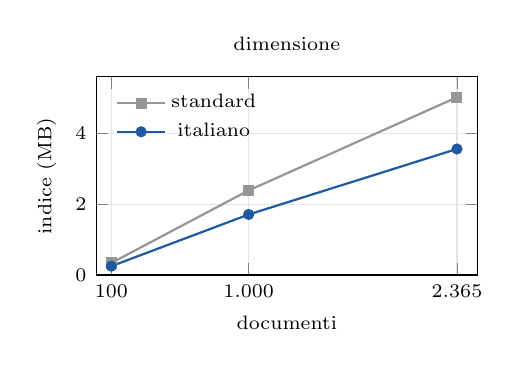
\begin{tikzpicture}
\begin{axis}[
  width=0.53\columnwidth, height=4.1cm,
  xlabel={documenti}, ylabel={indice (MB)},
  xmin=0, xmax=2500, ymin=0, ymax=5.6,
  xtick={100,1000,2365}, xticklabel style={font=\scriptsize},
  yticklabel style={font=\scriptsize}, label style={font=\scriptsize},
  /pgf/number format/use comma, scaled x ticks=false,
  legend style={font=\scriptsize,at={(0.03,0.97)},anchor=north west,draw=none,fill=none},
  grid=major, grid style={gray!20}, title={\scriptsize dimensione}]
\addplot[stdcol,thick,mark=square*,mark size=1.6pt] coordinates {(100,0.34) (1000,2.39) (2365,5.02)};
\addplot[itacol,thick,mark=*,mark size=1.6pt] coordinates {(100,0.25) (1000,1.71) (2365,3.56)};
\legend{standard, italiano}
\end{axis}
\end{tikzpicture}%
\hfill
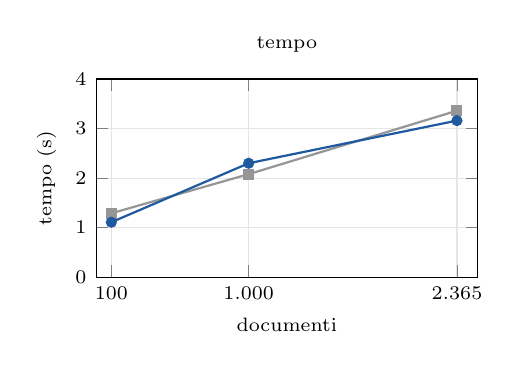
\begin{tikzpicture}
\begin{axis}[
  width=0.53\columnwidth, height=4.1cm,
  xlabel={documenti}, ylabel={tempo (s)},
  xmin=0, xmax=2500, ymin=0, ymax=4,
  xtick={100,1000,2365}, xticklabel style={font=\scriptsize},
  yticklabel style={font=\scriptsize}, label style={font=\scriptsize},
  /pgf/number format/use comma, scaled x ticks=false,
  grid=major, grid style={gray!20}, title={\scriptsize tempo}]
\addplot[stdcol,thick,mark=square*,mark size=1.6pt] coordinates {(100,1.29) (1000,2.08) (2365,3.36)};
\addplot[itacol,thick,mark=*,mark size=1.6pt] coordinates {(100,1.11) (1000,2.30) (2365,3.16)};
\end{axis}
\end{tikzpicture}
\caption{Dimensione dell'indice e tempo di indicizzazione al crescere del corpus.}
\label{fig:indice}
\end{figure}

Emergono tre osservazioni.
\begin{itemize}
  \item \textbf{Dimensione.} L'indice \emph{italiano} è più piccolo del 26--29\% a ogni scala: stopword e
        stemming riducono sia i termini distinti sia le posizioni da registrare.
  \item \textbf{Tempo.} Il tempo cresce molto meno che proporzionalmente ai documenti: una quota fissa di
        circa un secondo è dovuta all'avvio e al riscaldamento della JVM. Le differenze tra i due analyzer sono
        nell'ordine del rumore di misura.
  \item \textbf{Lanci a freddo.} In tre casi il primo lancio subito dopo la creazione dei file è stato molto
        più lento (19,2\,s, 35,9\,s e 23,7\,s), mentre il successivo sugli stessi file è tornato a 2--4\,s.
        La causa più probabile è la prima lettura dal disco di file appena scritti (cache del sistema
        operativo, scansione antivirus); questi lanci sono esclusi dalle medie.
\end{itemize}

\begin{table*}[t]
\centering\footnotesize
\caption{Query di test, con il numero di documenti rilevanti nel corpus (2365 documenti).}
\label{tab:query}
\begin{tabularx}{\textwidth}{@{}l>{\ttfamily}lXr@{}}
\toprule
\textbf{ID} & \textbf{\normalfont\bfseries Query} & \textbf{Bisogno informativo e aspetto verificato} & \textbf{Ril.} \\
\midrule
Q01 & nome commedia                      & Tutti i pezzi della Divina Commedia; tokenizzazione del nome del file. & 101 \\
Q02 & nome "promessi sposi"              & Tutti i pezzi dei Promessi sposi; phrase query sul nome. & 294 \\
Q03 & nome 042                           & Il pezzo n.\ 42 di ogni libro; i numeri devono restare cercabili. & 15 \\
Q04 & contenuto renzo                    & Documenti con \emph{Renzo}; caso di controllo senza varianti. & 134 \\
Q05 & contenuto burattino                & \emph{burattino/i}; singolare e plurale. & 64 \\
Q06 & contenuto cavallo                  & \emph{cavallo/i/a/e}; genere e numero. & 323 \\
Q07 & contenuto amore                    & \emph{amore, amori, amor}, anche elisi (\emph{l'amore}); elisione e troncamento. & 577 \\
Q08 & contenuto citta                    & \emph{città}, digitata senza accento; accenti. & 584 \\
Q09 & contenuto mangiare                 & 46 forme del verbo \emph{mangiare}; coniugazioni. & 258 \\
Q10 & contenuto "nel mezzo del cammin"   & Il verso iniziale dell'Inferno; phrase query con stopword. & 1 \\
Q11 & contenuto "ramo del lago di como"  & L'incipit dei Promessi sposi; phrase query più lunga. & 2 \\
Q12 & contenuto +guerra +pace            & Sia \emph{guerra} sia \emph{pace} (con plurali); operatore AND. & 80 \\
Q13 & contenuto guerra -pace             & \emph{guerra} ma non \emph{pace}; operatore NOT. & 314 \\
Q14 & contenuto pinocchio geppetto       & \emph{Pinocchio} o \emph{Geppetto}; OR e ordinamento. & 61 \\
\bottomrule
\end{tabularx}
\end{table*}

\begin{table*}[t]
\centering\footnotesize
\caption{Precision (P), recall (R) e $F_1$ per query, con le configurazioni \emph{standard} e \emph{italiano}.
In grassetto i valori migliori quando le due configurazioni differiscono.}
\label{tab:risultati}
\begin{tabular}{@{}l>{\ttfamily}lr ccc c ccc@{}}
\toprule
& & & \multicolumn{3}{c}{\textbf{standard}} & & \multicolumn{3}{c}{\textbf{italiano}} \\
\cmidrule{4-6}\cmidrule{8-10}
\textbf{ID} & \textbf{\normalfont\bfseries Query} & \textbf{Ril.} & P & R & $F_1$ && P & R & $F_1$ \\
\midrule
Q01 & nome commedia                     & 101 & 1,000 & 1,000 & 1,000 && 1,000 & 1,000 & 1,000 \\
Q02 & nome "promessi sposi"             & 294 & 1,000 & 1,000 & 1,000 && 1,000 & 1,000 & 1,000 \\
Q03 & nome 042                          &  15 & 1,000 & 1,000 & 1,000 && 1,000 & 1,000 & 1,000 \\
Q04 & contenuto renzo                   & 134 & 1,000 & 1,000 & 1,000 && 1,000 & 1,000 & 1,000 \\
Q05 & contenuto burattino               &  64 & 1,000 & 0,891 & 0,942 && 1,000 & \textbf{1,000} & \textbf{1,000} \\
Q06 & contenuto cavallo                 & 323 & 1,000 & 0,678 & 0,808 && 1,000 & \textbf{0,997} & \textbf{0,998} \\
Q07 & contenuto amore                   & 577 & 1,000 & 0,393 & 0,565 && 1,000 & \textbf{0,671} & \textbf{0,803} \\
Q08 & contenuto citta                   & 584 & 0,000 & 0,000 & 0,000 && 0,000 & 0,000 & 0,000 \\
Q09 & contenuto mangiare                & 258 & 1,000 & 0,484 & 0,653 && 1,000 & \textbf{0,547} & \textbf{0,707} \\
Q10 & contenuto "nel mezzo del cammin"  &   1 & \textbf{1,000} & 1,000 & \textbf{1,000} && 0,500 & 1,000 & 0,667 \\
Q11 & contenuto "ramo del lago di como" &   2 & 1,000 & 1,000 & 1,000 && 1,000 & 1,000 & 1,000 \\
Q12 & contenuto +guerra +pace           &  80 & 1,000 & 0,913 & 0,954 && 1,000 & \textbf{0,975} & \textbf{0,987} \\
Q13 & contenuto guerra -pace            & 314 & 0,993 & 0,895 & 0,941 && \textbf{0,994} & \textbf{0,994} & \textbf{0,994} \\
Q14 & contenuto pinocchio geppetto      &  61 & \textbf{1,000} & 1,000 & \textbf{1,000} && 0,984 & 1,000 & 0,992 \\
\midrule
\multicolumn{3}{@{}l}{\textbf{Media (14 query)}} & \textbf{0,928} & 0,804 & 0,847 && 0,891 & \textbf{0,870} & \textbf{0,868} \\
\multicolumn{3}{@{}l}{MAP / P@10}               & \multicolumn{3}{c}{0,804 \;/\; 0,807} && \multicolumn{3}{c}{\textbf{0,870} \;/\; 0,807} \\
\bottomrule
\end{tabular}
\end{table*}

% =================================================================
\section{Il programma di ricerca}
\cls{Ricerca} legge da console righe della forma
\[
\texttt{<campo> <termini>},\qquad \texttt{campo}\in\{\texttt{nome},\ \texttt{contenuto}\}.
\]
I termini vengono passati al \cls{QueryParser} di Lucene per il campo scelto, con lo stesso analyzer
dell'indice. Termini tra virgolette diventano una phrase query, più termini senza operatori sono in OR, e sono
ammessi \texttt{+} (obbligatorio) e \texttt{-} (escluso). Il ranking è quello predefinito, BM25~\cite{robertson2009}.
Per ogni query il programma mostra la query dopo l'analisi, il numero esatto di documenti trovati, il tempo di risposta e i primi $k$ risultati con
score, nome e libro. Le query non valide producono un messaggio senza interrompere il programma.
Un esempio reale, con l'indice \emph{italiano} (colonna \emph{libro} omessa):

\smallskip\noindent\begin{minipage}{\columnwidth}
\begin{lstlisting}
> contenuto "nel mezzo del cammin"
Query Lucene      : contenuto:"? mezzo ? cammin"
Documenti trovati : 2   (62.3 ms)
  1. [score 1.622]  divina-commedia-002.txt
  2. [score 1.622]  divina-commedia-061.txt
\end{lstlisting}
\end{minipage}\smallskip

\noindent
La riga \emph{Query Lucene} mostra l'effetto dell'analisi: le stopword \emph{nel} e \emph{del} sono state
eliminate e restano come posizioni vuote (\texttt{?}), mentre \emph{cammin} è già la radice. Analogamente, la
query \texttt{nome la divina commedia} restituisce i 101 pezzi del poema (\emph{la} non compare in nessun nome),
tutti con lo stesso score: ogni nome contiene \emph{divina} e \emph{commedia} una volta e ha la stessa
lunghezza, quindi BM25 assegna lo stesso punteggio.

% =================================================================
\section{Valutazione}

\subsection{Ground truth}
Per ciascuna delle 14 query (\cref{tab:query}) abbiamo scritto un bisogno informativo e un criterio di
rilevanza esplicito e indipendente da Lucene: un'espressione regolare sul nome del file, un insieme di forme
di una parola, una frase in posizioni consecutive, oppure forme da escludere. Le forme sono elencate a mano;
per \emph{mangiare}, per esempio, sono 46.

Lo script \file{ground\_truth.py} applica i criteri al corpus dopo una normalizzazione minima e dichiarata:
minuscolo e divisione su ogni carattere non alfanumerico (\emph{l'amore} contiene quindi \emph{amore}),
mantenendo gli accenti. Il ground truth descrive ciò che un utente vorrebbe trovare, non ciò che Lucene trova:
le metriche misurano quanto ciascun analyzer vi si avvicina.

\subsection{Metriche}
Per ogni query recuperiamo \emph{tutti} i documenti che la soddisfano, in ordine di score. Detti $\mathcal{R}$ i
documenti rilevanti e $\mathcal{A}$ quelli recuperati:
\[
P=\frac{|\mathcal{R}\cap\mathcal{A}|}{|\mathcal{A}|},\qquad
R=\frac{|\mathcal{R}\cap\mathcal{A}|}{|\mathcal{R}|},\qquad
F_1=\frac{2PR}{P+R}.
\]
Riportiamo inoltre la precision sui primi dieci risultati (P@10) e la \emph{mean average precision} (MAP). Le
medie sono \emph{macro}: ogni query pesa allo stesso modo.

\subsection{Risultati}
La \cref{tab:risultati} riporta le metriche per query; la \cref{fig:recall} confronta la recall sulle query in cui
contano le varianti delle parole.

\begin{figure}[t]
\centering
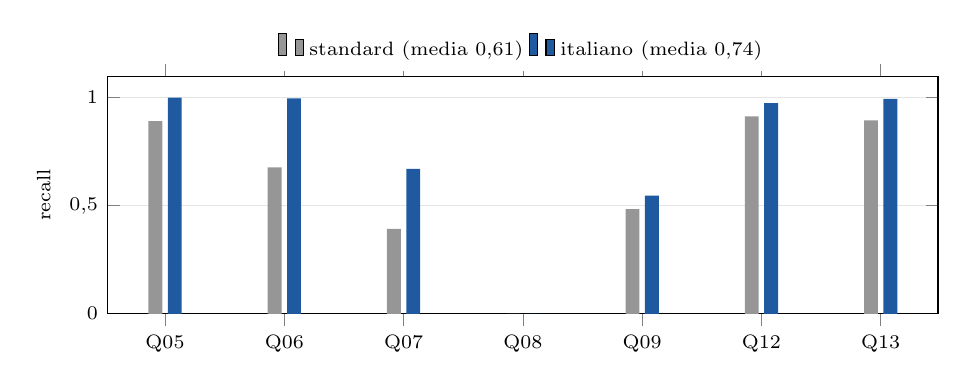
\begin{tikzpicture}
\begin{axis}[
  ybar, bar width=5pt, width=\columnwidth, height=4.6cm,
  ymin=0, ymax=1.1, ylabel={recall}, label style={font=\scriptsize},
  symbolic x coords={Q05,Q06,Q07,Q08,Q09,Q12,Q13},
  xtick=data, tick label style={font=\scriptsize},
  /pgf/number format/use comma,
  legend style={font=\scriptsize,at={(0.5,1.02)},anchor=south,legend columns=2,draw=none},
  ymajorgrids, grid style={gray!20}, enlarge x limits=0.08]
\addplot[fill=stdcol,draw=none] coordinates {(Q05,0.891) (Q06,0.678) (Q07,0.393) (Q08,0) (Q09,0.484) (Q12,0.913) (Q13,0.895)};
\addplot[fill=itacol,draw=none] coordinates {(Q05,1.000) (Q06,0.997) (Q07,0.671) (Q08,0) (Q09,0.547) (Q12,0.975) (Q13,0.994)};
\legend{{standard (media 0,61)},{italiano (media 0,74)}}
\end{axis}
\end{tikzpicture}
\caption{Recall sulle sette query in cui contano le varianti delle parole.}
\label{fig:recall}
\end{figure}

\subsection{Discussione}
\paragraph{Effetto complessivo.} \cls{ItalianAnalyzer} aumenta la recall media da 0,804 a 0,870 e la $F_1$ da 0,847
a 0,868, con un calo di precision da 0,928 a 0,891: è il compromesso atteso dallo stemming. Nelle medie
l'effetto è diluito dalle query su cui entrambe le configurazioni sono perfette; sulle sette query sensibili alle
varianti la recall media sale da 0,61 a 0,74.

\paragraph{Nome e controllo (Q01--Q04).} Risultati perfetti per entrambe: il campo nome usa lo stesso
analyzer, e la tokenizzazione su trattini e punti consente ricerche per titolo, frase e numero. Q04 conferma
che, senza varianti, i due analyzer si equivalgono.

\paragraph{Singolare e plurale (Q05, Q06, Q12, Q13).} È l'effetto più netto: \cls{StandardAnalyzer} perde i
documenti che contengono solo il plurale (recall 0,68 su \emph{cavallo}), \cls{ItalianAnalyzer} li recupera quasi
tutti (0,997).

\paragraph{Elisioni (Q07).} \cls{StandardAnalyzer} tratta \emph{l'amore} come un unico token e si ferma a 0,39;
\cls{ItalianAnalyzer} rimuove gli articoli elisi e arriva a 0,67. I documenti mancanti contengono probabilmente
elisioni assenti dall'elenco di Lucene, frequenti in poesia (\emph{ch'amor}, \emph{quell'amore}): è
un'ipotesi da verificare.

\paragraph{Accenti (Q08).} Nessuna delle due configurazioni trova documenti se l'utente scrive \emph{citta} senza
accento. Contrariamente alle attese, lo stemmer italiano non normalizza gli accenti: servirebbe un filtro
dedicato come \cls{ASCIIFoldingFilter}.

\paragraph{Coniugazioni (Q09).} Il guadagno è minimo (da 0,48 a 0,55): lo stemming leggero non unifica le forme
verbali (\emph{mangiò}, \emph{mangerà}, \emph{mangiando}); servirebbero uno stemmer più aggressivo o la
lemmatizzazione.

\paragraph{Frasi e stopword (Q10, Q11).} Con \cls{ItalianAnalyzer} la frase \emph{nel mezzo del cammin} diventa
\emph{mezzo \_ cammin}. Oltre al verso iniziale dell'Inferno, corrisponde a un verso del canto XXVI del Purgatorio,
\emph{``ché per lo mezzo del cammino acceso''}: \emph{del} è eliminata come stopword e lo stemming riduce
\emph{cammino} a \emph{cammin}. La precision scende così a 0,5: per le citazioni esatte \cls{StandardAnalyzer}
è più adatto.

\paragraph{Errori comuni (Q13, Q14).} In Q13 entrambe le configurazioni recuperano due documenti non rilevanti:
la causa va quindi cercata nella tokenizzazione, comune alle due configurazioni, più che nello stemming. Un'ipotesi è il corsivo di Gutenberg
(\texttt{\_pace\_}), che il tokenizer unisce alla parola. In Q14 \cls{ItalianAnalyzer} recupera un documento non
rilevante in più, forse per la confusione tra \emph{Pinocchio} e i \emph{pinocchi} (pinoli) dell'Artusi.

\paragraph{Note sulle metriche.} P@10 vale 0,1 e 0,2 in Q10 e Q11 solo perché esistono 1 e 2 documenti
rilevanti. L'AP coincide con la recall quando tutti i recuperati sono rilevanti, perché la precision vale 1 in
ogni posizione.

% =================================================================
\section{Limiti e sviluppi futuri}
\begin{itemize}
  \item Il ground truth è \emph{lessicale}: non considera documenti che trattano l'argomento con altre parole
        (\emph{destriero} per \emph{cavallo}). Ciò spiega anche la precision quasi sempre pari a 1.
  \item Le ipotesi su Q07, Q13 e Q14 andrebbero verificate elencando documenti mancati e falsi positivi.
  \item I risultati suggeriscono un terzo analyzer: \cls{ItalianAnalyzer} con \cls{ASCIIFoldingFilter} e un elenco
        esteso di elisioni, da valutare sulle stesse query.
  \item I tempi sono piccoli e sensibili ad avvio della JVM e cache del disco: servirebbero un corpus più grande
        e più ripetizioni.
\end{itemize}

% =================================================================
\section{Conclusioni}
Il sistema indicizza 2365 documenti in circa 3 secondi e risponde alle query in qualche decina di
millisecondi al più. Per testi in
italiano \cls{ItalianAnalyzer} è la scelta migliore per il campo contenuto: indice più piccolo del 26--29\% e
recall più alta sulle varianti delle parole, al prezzo di una lieve perdita di precision sulle frasi esatte. Per
il campo nome, uno \cls{StandardAnalyzer} che separa su trattini e punti consente ricerche per parola, frase e
numero. I casi scoperti (accenti, coniugazioni, elisioni poetiche) indicano con chiarezza le estensioni da
provare.

% =================================================================
\section*{Riproducibilità}
Il codice, i risultati e questa relazione sono nel repository indicato in testa. Dalla cartella del progetto:
\begin{lstlisting}
python scripts/prepara_corpus.py
Indicizzatore corpus/completo indice/completo-italiano italiano
Indicizzatore corpus/completo indice/completo-standard standard
python scripts/ground_truth.py
Ricerca       indice/completo-italiano italiano
Valutazione   docs/query.tsv docs/qrels.csv docs indice/completo-standard
              standard indice/completo-italiano italiano
\end{lstlisting}
Le classi Java si eseguono da Eclipse (\emph{Run Configurations}) con gli argomenti indicati. Le misure grezze dei tempi sono in
\file{docs/tempi\_indicizzazione.csv}, i risultati in \file{docs/valutazione.csv}.

% =================================================================
\begin{thebibliography}{9}
\footnotesize\setlength{\itemsep}{1pt}\setlength{\parskip}{0pt}
\bibitem{lucene} Apache Software Foundation. \emph{Apache Lucene}. \url{https://lucene.apache.org/}.
\bibitem{gutenberg} Project Gutenberg. \url{https://www.gutenberg.org/}.
\bibitem{manning2008} C.~D. Manning, P.~Raghavan, H.~Schütze. \emph{Introduction to Information Retrieval}.
  Cambridge University Press, 2008.
\bibitem{robertson2009} S.~Robertson, H.~Zaragoza. The Probabilistic Relevance Framework: BM25 and Beyond.
  \emph{Foundations and Trends in Information Retrieval}, 3(4):333--389, 2009.
\end{thebibliography}

\end{document}
